\subsection{Offene Punkte}
\label{offenepunkte}
\textit{(ygu/pro)} Die Inbetriebnahme musste aus Zeitgründen frühzeitig beendet werden. Jede Teilkomponente konnte grundlegend getestet werden, für eine vollumfängliche Funktionserfüllung ist jedoch eine weitere, vertiefte Inbetriebnahme nötig.
\newline

In diesem Unterkapitel sind Punkte aufgeführt, welche noch unbehandelt sind. Dabei wird unterschieden in Punkte:
\begin{itemize}
	\item Die zur vollumfänglichen Erfüllung des Pflichtenhefts noch erledigt werden müssen (to-do). 
	
	\item Welche die Performance und Handhabung des Planting Robots verbessern (nice to have). 
\end{itemize}

\textbf{to-do:}
\begin{itemize}
	\item Die Parameter der Verstellmechanik müssen gemäss den verschiedenen Setzradien ermittelt und in der Software geändert werden.
	\item Die Software muss um eine adäquate Topferkennung erweitert werden. Die Sensoranbindung für einen IR-Sensor ist dabei schon implementiert.
	\item Entsprechend der Topferkennung muss die FSM erweitert werden, sodass der Setzprozess bei erkanntem Topf ausgelöst wird.
	
	\item Das Ausheben der Setzlöcher mit der vorgegebenen Topferde ist zu untersuchen.
	
	\item Das Zusammenspiel aller Teilfunktionen muss umfassend getestet werden. Dabei kann in einem ersten Schritt mit der realisierten Testumgebung der Prozess simuliert werden.
	
	\item In einem letzten Schritt ist das Funktionsmuster an der Topfmaschine in Betrieb zu nehmen.
\end{itemize}

\textbf{nice to have:}
\begin{itemize}
	\item Die verwendeten PID Positionierungsregler für die Setzeinheit, Verstellmechanik und Setzeinheit könnten optimiert werden. Dafür müssten die Sprungantworten der jeweiligen Strecken ermittelt und über ein entsprechendes mathematisches Modell approximiert werden. Auf Grundlage der Strecke könnten dann die Parameter für den Regler definiert werden.
	\item Die Initialisierung der Setzeinheit könnte erweitert werden, indem die Setzeinheit nach erreichen des oberen Endanschlags bis an den unteren Anschlag fährt. Die dabei zurückgelegte Strecke könnte mit der tatsächlichen Länge der Spindel verglichen werden. Durch diesen Vergleich würde sichergestellt, dass die Setzeinheit nicht durch äussere Einflüsse (wie eine verschmutzte Spindel) fälschlicherweise einen Endanschlag vermutet.
	\item Der qualitativ durchschnittliche Antrieb (Pololu 25D) durch einen qualitativ besseren Motor ersetzen, welcher ein geringeres Spiel aufweist.
	\item Die Anordnung des Antriebs neu konzipieren. Dabei kann das Spiel massiv reduziert werden, indem der Antrieb an der Aussenkontur der Lochmaske gekoppelt wird. Dabei muss an der Aussenkontur eine Verzahnung realisiert werden, sodass über ein zweites Zahnrad der Motor die Rotation umsetzen kann (siehe Abbildung \ref{fig:optimierung_lochmaske}). Die Grössenordnung dieser Übersetzung ist variabel, führt jedoch bei optimaler Auslegung dazu, dass ein Antrieb mit geringerer Übersetzung verwendet werden kann. Dadurch wird das Spiel reduziert. 
\end{itemize}

\begin{figure}[H]
	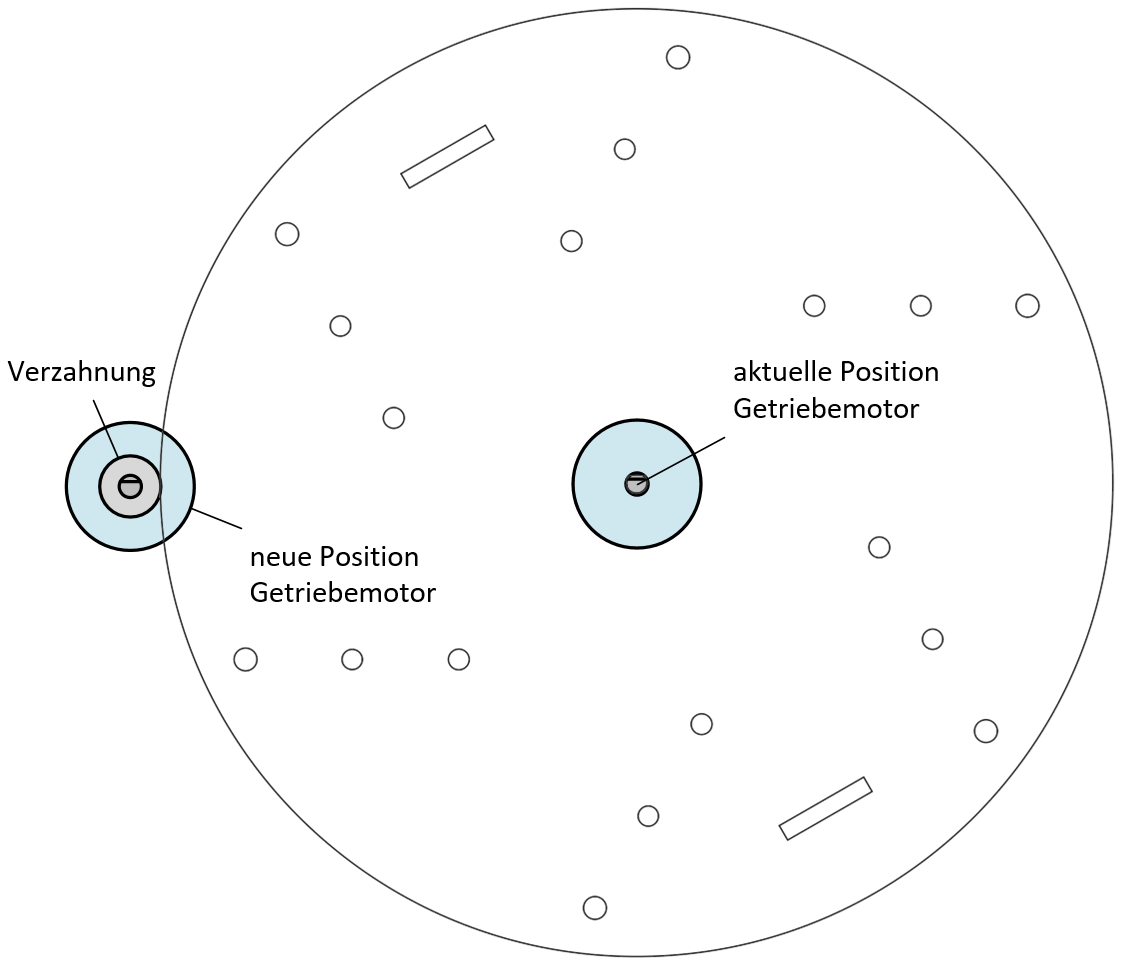
\includegraphics[draft=false,scale=0.4]{Illustrationen/8-Fazit/optimierung_lochmaske.png}
	\caption{verbesserte Anordnung des Antriebs für die Lochmaske}
	\label{fig:optimierung_lochmaske}
\end{figure}